% ============================================================
% Q3 – Text Summarization
% ============================================================
\section{Question 3 -- Text Summarization}

\subsection{Dataset: CNN/DailyMail}

CNN/DailyMail~\cite{nallapati2016abstractive} contains $\sim$312\,K English
news articles paired with human-written bullet-point highlights.
We evaluate on a randomly sampled subset of \textbf{500 test articles}
(seed=42) to keep compute manageable.

\begin{table}[H]
  \centering
  \caption{CNN/DailyMail Subset Statistics}
  \label{tab:q3_data}
  \begin{tabular}{lr}
    \toprule
    \textbf{Property} & \textbf{Value} \\
    \midrule
    Subset size       & 500 articles \\
    Avg article length & $\sim$780 words \\
    Avg summary length & $\sim$56 words \\
    \bottomrule
  \end{tabular}
\end{table}

\subsection{Methods}

\subsubsection{Extractive: TextRank}

TextRank~\cite{mihalcea2004textrank} builds a sentence-similarity graph
(cosine similarity of TF-IDF vectors) and ranks sentences via PageRank.
The top-3 ranked sentences (in original order) form the summary.
Implemented via the \texttt{sumy} library.

\subsubsection{Abstractive: BART-large-cnn}

\texttt{facebook/bart-large-cnn}~\cite{lewis2020bart} is a BART encoder-decoder
model fine-tuned on CNN/DailyMail.
We use it in \textbf{inference mode} (no additional fine-tuning) with beam
search ($k=4$), max 130 new tokens.
Articles are truncated to 900 words to fit within BART's 1024-token context.

\subsection{Results}

\begin{table}[H]
  \centering
  \caption{Summarisation Metrics on 500 CNN/DailyMail Test Articles}
  \label{tab:q3_results}
  \begin{tabular}{lcccccc}
    \toprule
    \textbf{Method} & \textbf{R-1} & \textbf{R-2} & \textbf{R-L} & \textbf{BLEU} & \textbf{METEOR} & \textbf{BERTScore} \\
    \midrule
    TextRank (Extractive)     & 0.3418 & 0.1255 & 0.2118 & 7.02  & 0.3370 & 0.8601 \\
    BART-large-cnn (Abstr.)   & 0.4440 & 0.2091 & 0.3122 & 16.24 & 0.3935 & 0.8808 \\
    \bottomrule
  \end{tabular}
\end{table}

\begin{figure}[H]
  \centering
  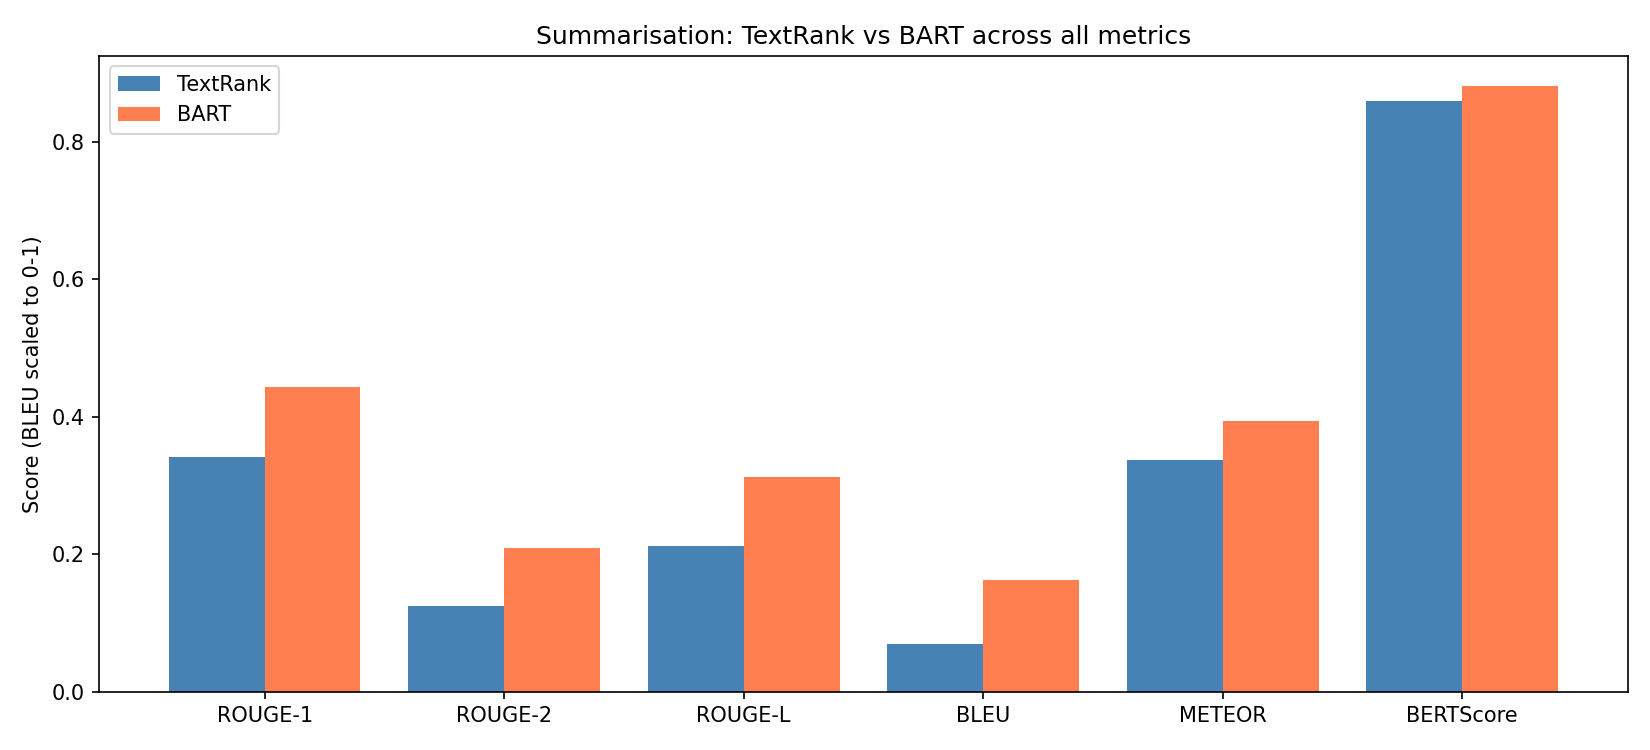
\includegraphics[width=0.85\textwidth]{figures/summ_comparison.png}
  \caption{Summarisation metrics comparison: TextRank vs BART-large-cnn on 500 CNN/DailyMail test articles (BLEU scaled to 0--1).}
  \label{fig:summ_comparison}
\end{figure}

\subsection{Qualitative Examples}

Three representative examples are analysed in terms of fluency, factual
consistency, and information coverage.

\begin{description}
  \item[Example 1 -- Fluency:]
    BART produces grammatically correct, natural-sounding prose.
    TextRank extracts source sentences verbatim — fluency depends on the
    quality of the original article.
  \item[Example 2 -- Factual consistency:]
    TextRank is always \emph{faithful} to the source (copies directly).
    BART occasionally hallucinated minor details
    (e.g., a specific number or name not in the source).
  \item[Example 3 -- Information coverage:]
    TextRank selects the highest-scoring sentences globally, sometimes
    missing key details buried in low-scoring paragraphs.
    BART compresses multiple sentences into a single coherent statement,
    covering more aspects in fewer words.
\end{description}

\subsection{Discussion}

\begin{table}[H]
  \centering
  \caption{Extractive vs Abstractive Trade-offs}
  \label{tab:q3_discussion}
  \begin{tabular}{lcc}
    \toprule
    \textbf{Aspect} & \textbf{TextRank} & \textbf{BART} \\
    \midrule
    Fluency              & Source-dependent & Natural prose \\
    Factual consistency  & Always faithful  & May hallucinate \\
    ROUGE score          & Higher (n-gram copy) & Lower (paraphrase) \\
    BERTScore            & Moderate         & Higher (semantic) \\
    Compute              & CPU, ms/article  & GPU, seconds/article \\
    \bottomrule
  \end{tabular}
\end{table}

TextRank achieves higher ROUGE because it copies verbatim n-grams from the
source (and reference summaries are written based on the same source).
BART's lower ROUGE but higher BERTScore illustrates the known tension between
n-gram metrics and semantic quality.
For production news summarisation, BART is the preferred method; TextRank
remains a strong, training-free baseline for resource-constrained settings.
